\documentclass{article}
\usepackage[margin=2cm]{geometry}

\usepackage{amsmath, amssymb, amsthm}
\usepackage{fancyhdr}
\usepackage{pgfplots}

\begin{document}

\begin{figure}
\centering
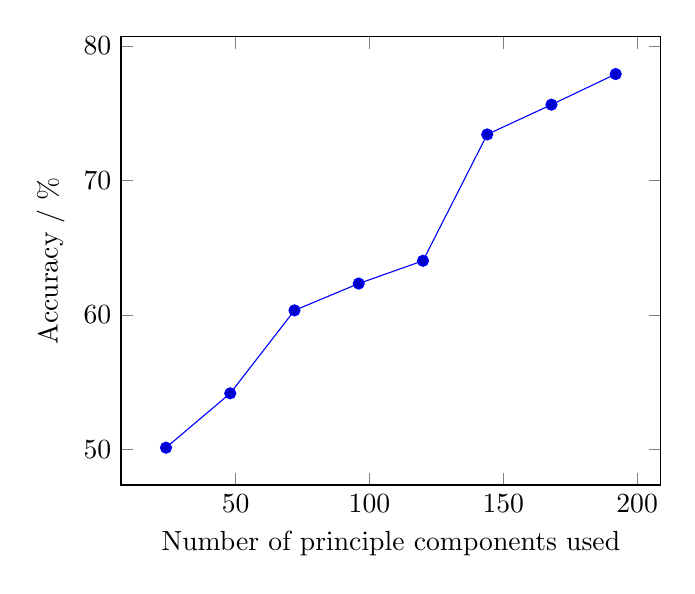
\begin{tikzpicture}
  \begin{axis}[
      xlabel={Number of principle components used},
      ylabel={Accuracy / \%}]
    ]
      \addplot coordinates {
        (24, 50.14)
        (48, 54.177)
        (72, 60.341)
        (96, 62.334)
        (120, 64.027)
        (144, 73.415)
        (168, 75.628)
        (192, 77.9)
      };
  \end{axis}
\end{tikzpicture}
\caption{Using PCA to perform dimension reduction is not always a good idea. }
\end{figure}

\begin{figure}
\label{tabAcc}
\centering
\begin{tabular}{|c|c|}
  \hline
  \textbf{Method} & \textbf{Accuracy}\\
  \hline
  Random & 10.0\%\\
  Raw pixels & 37.3\%\\
  K-means + all PCs & 77.9\%\\
  K-means + 0.99 variance & 50.0\%\\
  3 layers & 82.0\%\\
  Sparse 3 layers & 83.5\%\\
  \hline
\end{tabular}
\end{figure}

\begin{figure}
\label{figSparseKM}
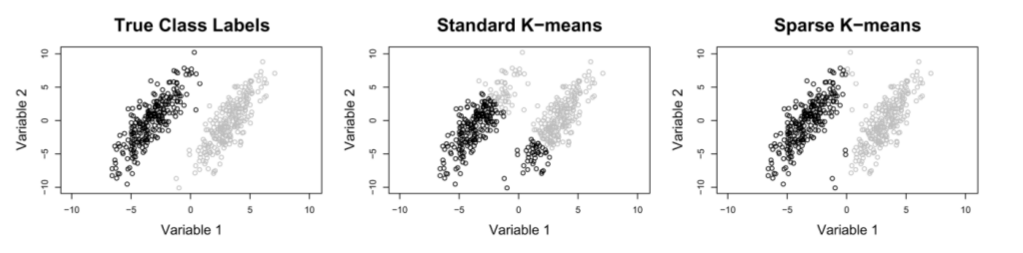
\includegraphics[width=\columnwidth]{./sparse.png}
\caption{Sparse K-means helps us perform feature selection}
\end{figure}
Figure \ref{tabAcc} shows the accuracy of different algorithms with all 50000 training examples from CIFAR-10. The algorithms were

\subsection{Sparse K-Means}

K-means is not by default robust to non-discriminative features. Specifically, if we have a lot of features that will not help us to seperate different classes, then those features will actually hurt the clustering algorithm. This problem is shown in figure (sparse classed k-means). Here, we notice that the second feature does not help us to determine which class a point belongs to. Worse, in this case it actually changes the assignment of the clusters. We want to remove these features from consideration.

\begin{itemize}
\item[1.] randomly choosing a class.
\item[2.] Taking the raw pixels from each image and feeding them into an SVM
\item[3.] Single layer K-means we have described above.
\item[4.] K-means with PCA run on the patches, keeping 99\% of the variance.
\item[5.] Stacking the K-means feature learner into a deep network.
\item[6.] 3-layer network, but we use sparse K-means at the deeper levels.
\end{itemize}
Running an SVM against raw pixels shows us that raw pixels do not make for a good feature representation for image classification.

Running PCA on image patches also sacrifices a large amount of accuracy. If we were to run PCA on the data in Figure \ref{figSparseKM} we would not be able to get good clusters on the new space. This is reflected in the accuracy drop from using PCA based on the total variance of the data.

\end{document}
